\section{Results}
\label{sec:results}
%
The newly developed code was used to carry out some numerical experiments which are presented in this section.
Aspects that need to be checked are the correctness of the propagators from a quantum mechanical point of view (subsection~\ref{subsec:physical}), convergence of the methods (subsection~\ref{subsec:convergence}) and benchmarking of the compute time (subsection~\ref{subsec:benchmark}).
\par\medskip
%
The potentials used for these numerical experiments are the harmonic, torsional and Morse potential that are now briefly introduced.
The value $\eps = 0.01$ was used if not specified otherwise.


\paragraph{Harmonic Potential}
The generalized harmonic potential
\begin{align}
	\label{math:harmonic}
	V(\bvec{x}) = \frac{1}{2} \sum_{i=1}^D x_i^2
\end{align}
%
was used with initial values $\bvec{q} = (1,\dots,1)^T$, $\bvec{q} = (1,\dots,1,-1,\dots,-1)$, $\bmat{Q}$ and $\bmat{P} = \im \bmat{Q}^{-1}$. \\
\par\medskip


\paragraph{Torsional Potential}
The torsional potential
%
\begin{align}
	\label{math:torsional}
	V(\bvec{x}) = \sum_{i=1}^D \left( 1 - \cos x_i \right)
\end{align}
%
was used with initial values $\bmat{Q} = \bmat{I}_N$, $\bmat{P} = \im \bmat{I}_N$, $\bvec{q} = (1,0,\dots,0)$ and $\bvec{p} = (0,\dots,0)$ as suggested in \cite{FGL_semiclassical_dynamics}.

\paragraph{Morse Potential}
%
The Morse potential was also used for numerical experiments in \cite{Unpublished} and looks as follows:
%
\begin{align}
	\label{math:morse}
	V(\bvec{x}) = C e^{-2a(x-x_0)} - 2 e^{-a(x-x_0)} \; .
\end{align}
%
Where $C = 0.004164$, $a=0.896696$, $x_0 = 5.542567$ are constants.
For this 1D potential, the physically correct parameters $q_0 = 6.0426$, $p_0 = -0.1100$, $Q_0 = 3.4957$, $P_0 = 0.2861 \im$ with $\eps = 0.0484$ was used for all simulations.



\subsection{Physical Correctness}
\label{subsec:physical}
%
In order to analyze the physical correctness of the implemented propagators, a two dimensional wave packet was propagated in the Harmonic potential and in the Henon-Heiles potential presented above with each of the presented propagators for a time $T = 10$ with timestep $\Dt = 0.01$.
All propagators used the \emph{LT} splitting coefficients for the \proc{IntSplit} method.
\par\medskip
%
Figure \ref{fig:energy_Semiclassical} shows the time evolution of energy and the energy drift for the semiclassical propagator. The corresponding energy plots for the remaining propagators can be found in the appendix to the report.
The equivalent conservation plot for the two dimensional case is shown in figure \ref{fig:energy_Semiclassical_2D}. \\
As is clearly shown by the graphs, the propagators conserve the total energy (apart from very small oscillations).
%
\begin{figure}[ht]
	\centering
	\begin{minipage}[c]{\textwidth}
		\begin{center}
			\large Semiclassical Propagator \\[1mm]
			\normalsize Energy Evolution and Drift
			\vspace{4mm}
		\end{center}
	\end{minipage}
	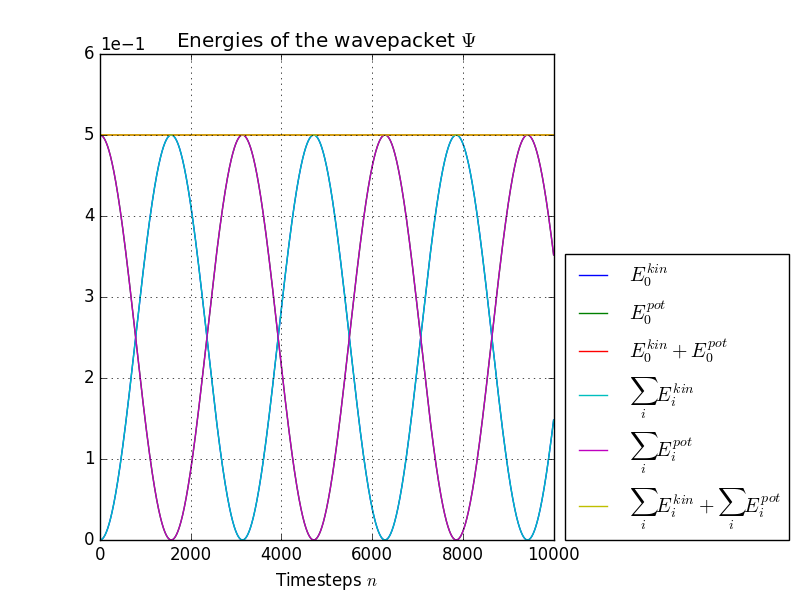
\includegraphics[width=.45\textwidth]{figures/harmonic_1D_Semiclassical_energies.png}
	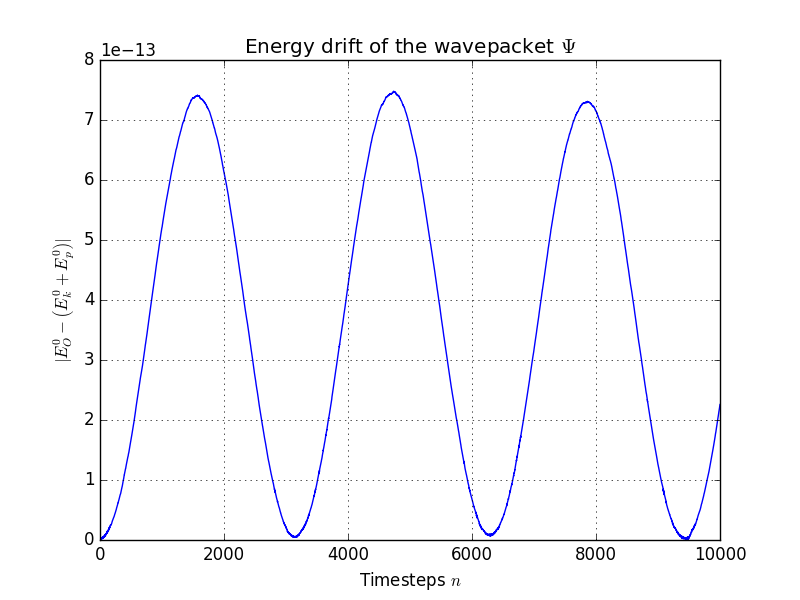
\includegraphics[width=.45\textwidth]{figures/harmonic_1D_Semiclassical_drift.png} \\
	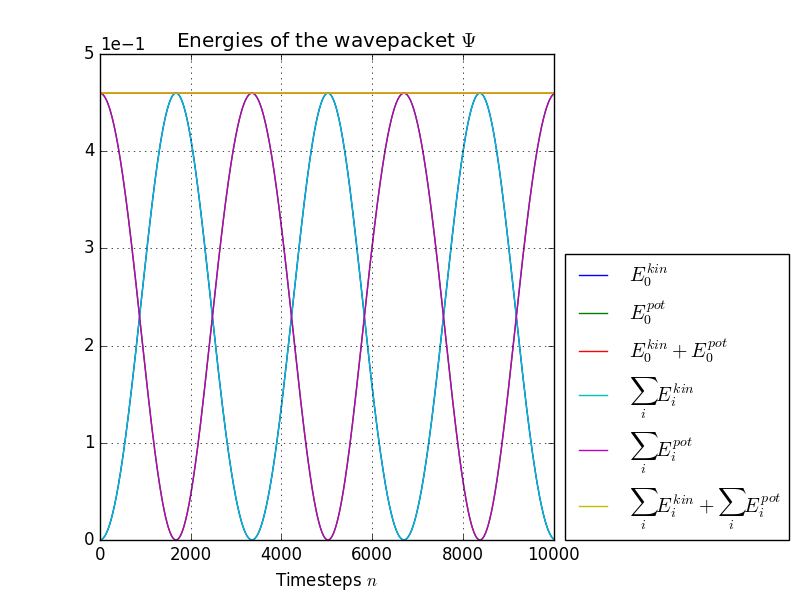
\includegraphics[width=.45\textwidth]{figures/torsional_1D_Semiclassical_energies.png}
	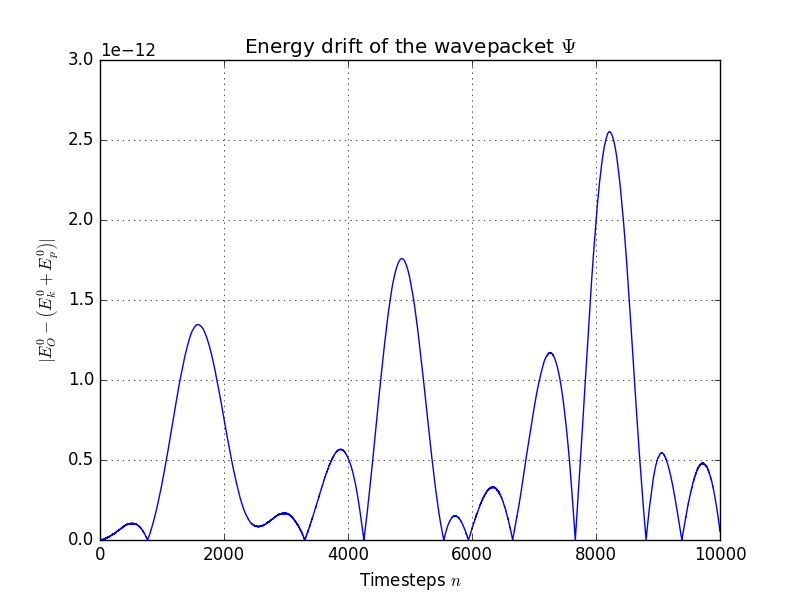
\includegraphics[width=.45\textwidth]{figures/torsional_1D_Semiclassical_drift.png} \\
	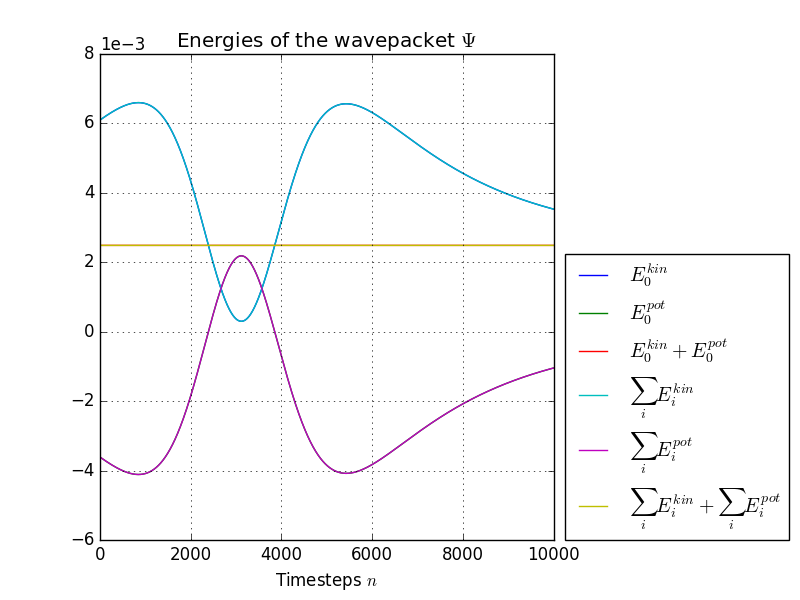
\includegraphics[width=.45\textwidth]{figures/morse_1D_Semiclassical_energies.png}
	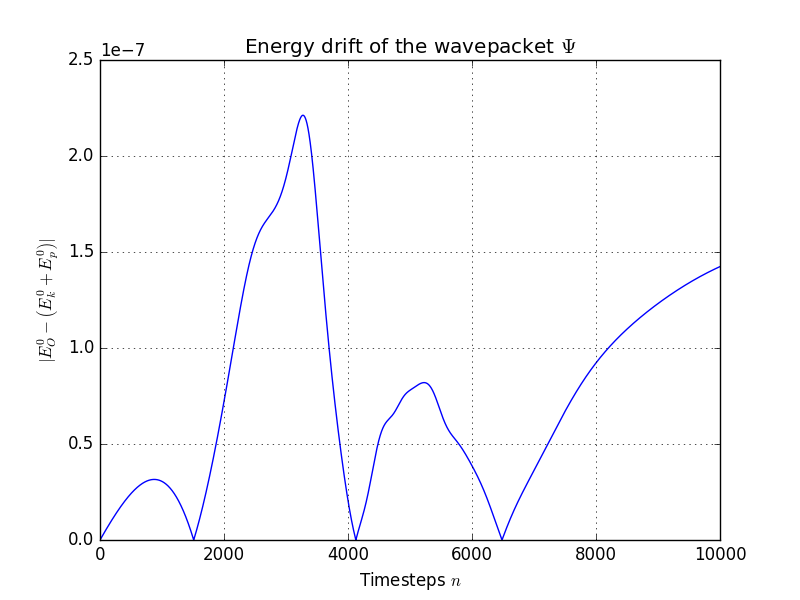
\includegraphics[width=.45\textwidth]{figures/morse_1D_Semiclassical_drift.png}
	\caption{Energy evolution and drift for a 1D wave packet propagated with the Semiclassical propagator in a harmonic potential (top), a torsional potential (middle) and a Morse potential (bottom).
	(Parameters: $N=1$, $D=1$ $|\K|=16$ $\eps=0.01$ (Morse $0.0484$), $T=10$ (Morse $T=50$), $\Dt=0.001$ (Morse $\Dt=0.005$), Semiclassical propagator with \emph{Y4} splitting for \proc{IntSplit})}
	\label{fig:energy_Semiclassical}
\end{figure}
%
\begin{figure}[ht]
	\centering
	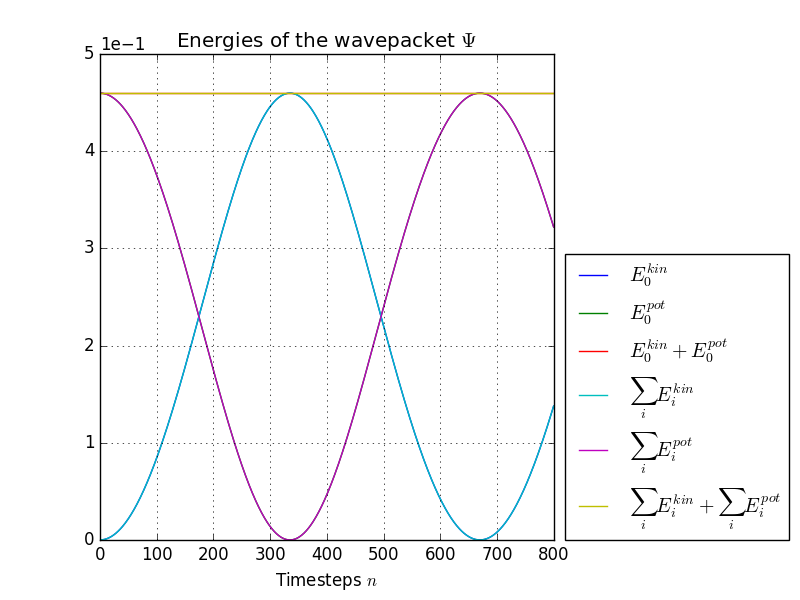
\includegraphics[width=.8\textwidth]{figures/torsional_2D_Semiclassical_energies.png}
	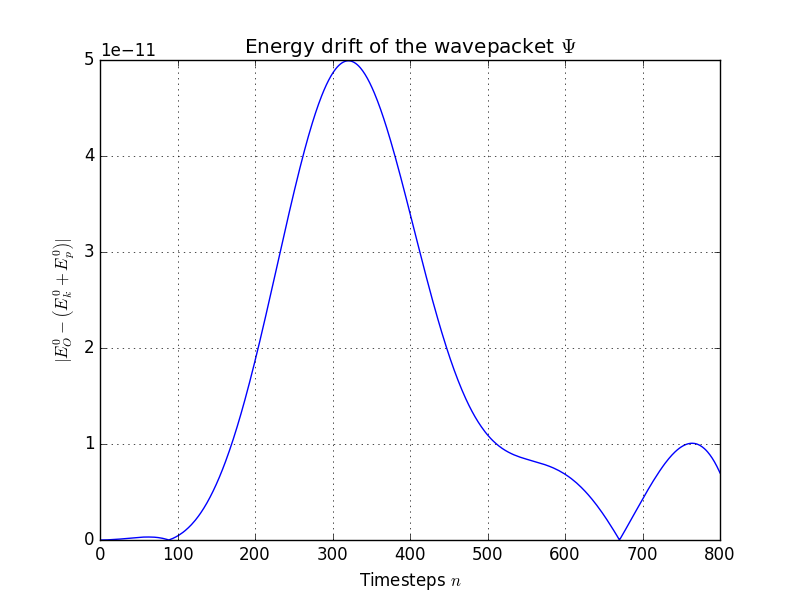
\includegraphics[width=.8\textwidth]{figures/torsional_2D_Semiclassical_drift.png}
	\caption{Energy evolution and drift for a wave packet propagated with the Semiclassical propagator in a 2D torsional potential.
	(Parameters: $N=1$, $D=2$ $|\K|=16$ $\eps=0.01$, $T=4$, $\Dt=0.005$, Semiclassical propagator with \emph{KL10} splitting for \proc{IntSplit})}
	\label{fig:energy_Semiclassical_2D}
\end{figure}


\subsection{Effect of Stepsize}
\label{subsec:convergence}
%
A convergence analysis was carried out in which the error of each propagator was recorded while reducing the stepsize $\Dt$.
A Semiclassical propagator with \emph{KL10} splitting coefficients and step size $\Dt = 0.0001$ was used to propagate the wave packet to a final time $T = 10$ and create a reference solution.
\par\medskip
%
The error between two wave packets was computed by evaluating them on a grid with 1000 grid points and taking the $L_2$ norm of the differences.
Figure \ref{fig:error_analysis} shows the error for different step sizes $\Dt$.
It is quite surprising how the Hagedorn Propagator has higher precision than the other schemes in the case of \emph{LT} splitting.
Only for higher order splitting coefficients like \emph{Y4} the advantages of \proc{IntSplit} start paying off and the other propagators show their advantages over the simplistic Hagedorn Propagator.
%
\begin{figure}[ht]
	\centering
	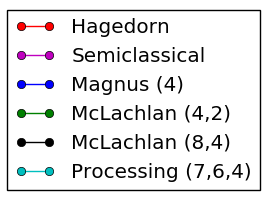
\includegraphics[width=.2\textwidth]{figures/convergence_legend.png} \\
	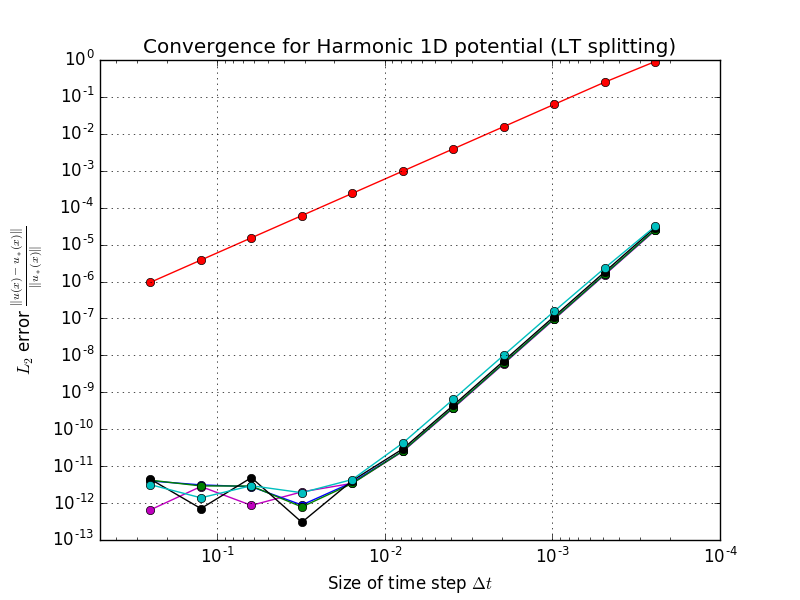
\includegraphics[width=.45\textwidth]{figures/convergence_harmonic_1D_lt.png}
	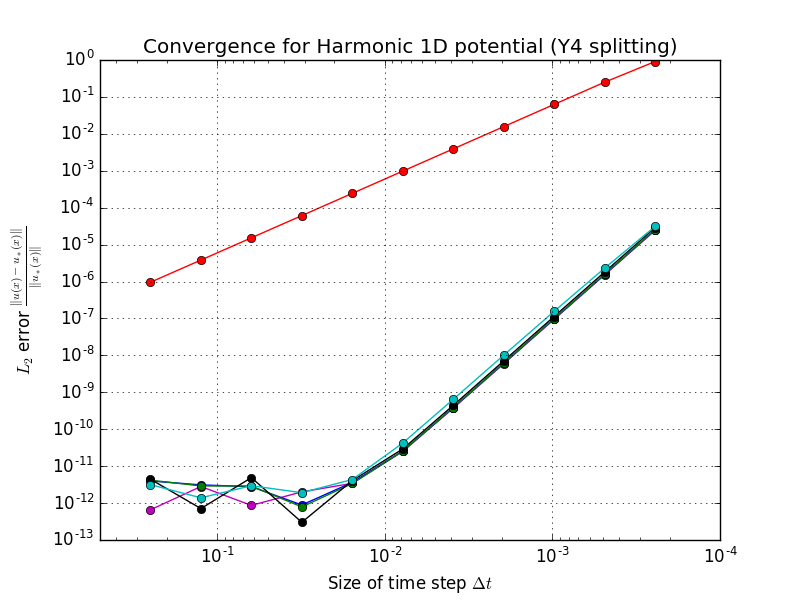
\includegraphics[width=.45\textwidth]{figures/convergence_harmonic_1D_y4.png} \\
	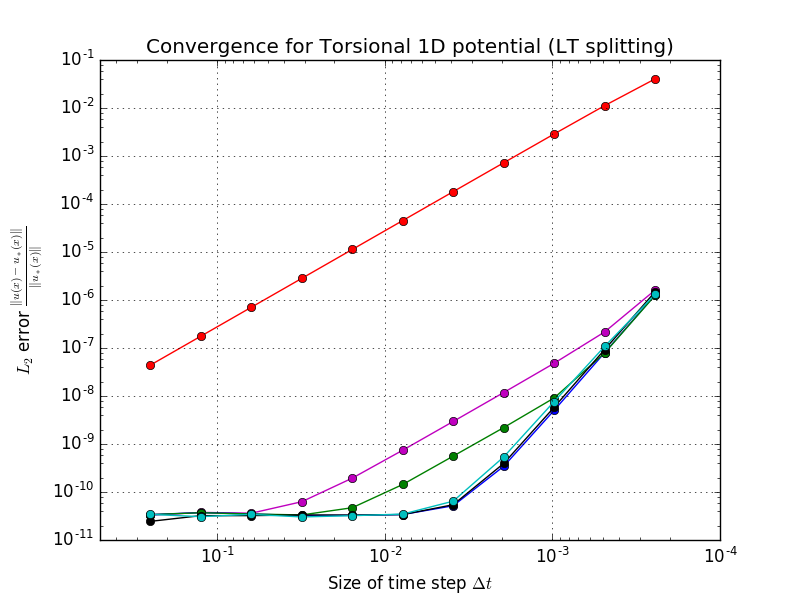
\includegraphics[width=.45\textwidth]{figures/convergence_torsional_1D_lt.png}
	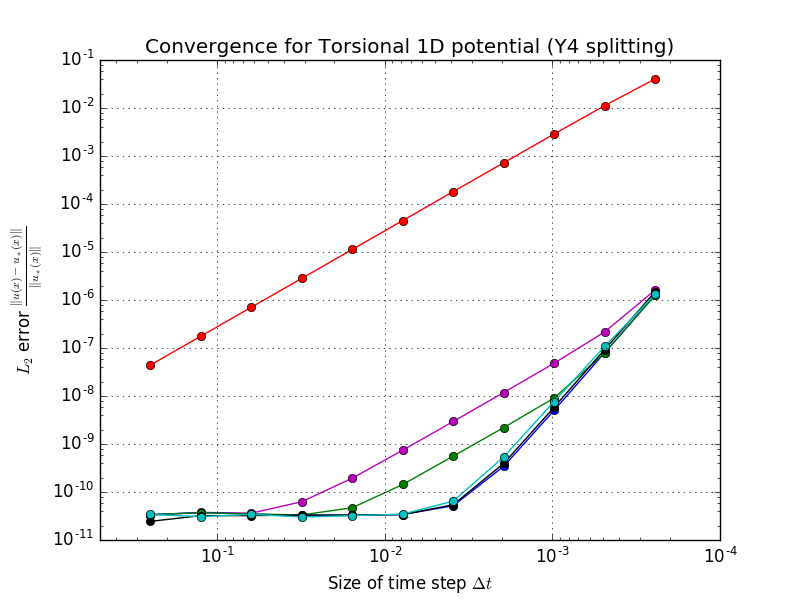
\includegraphics[width=.45\textwidth]{figures/convergence_torsional_1D_y4.png} \\
	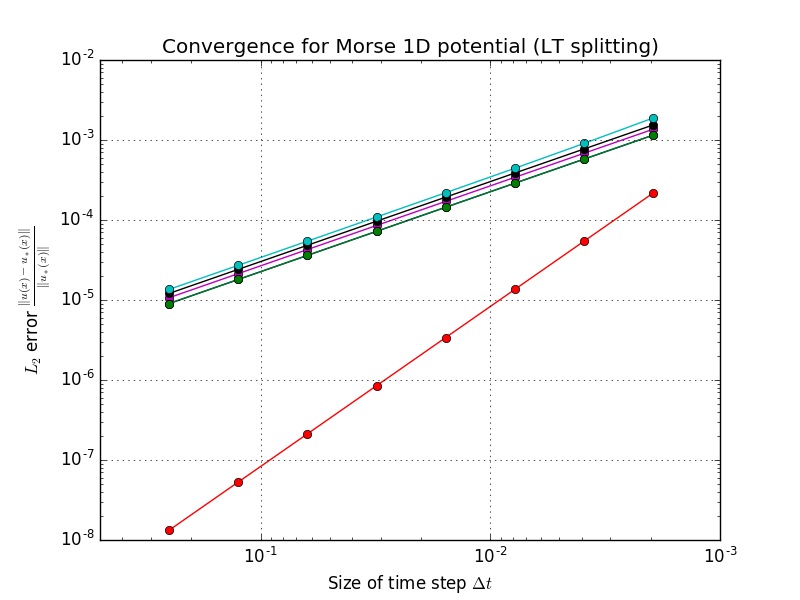
\includegraphics[width=.45\textwidth]{figures/convergence_morse_1D_lt.png}
	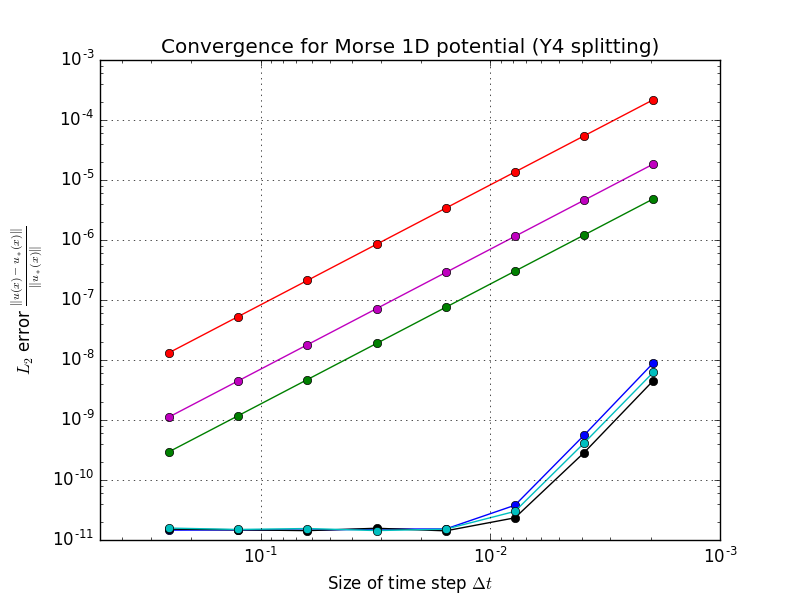
\includegraphics[width=.45\textwidth]{figures/convergence_morse_1D_y4.png}
	\caption{Convergence of the various propagators towards the reference solution for \emph{LT} splitting (left) and \emph{Y4} splitting (right). The potentials are the harmonic potential (top), the torsional potential (middlt) and the morse potential (bottom). The $L_2$ norm was measured by projecting the wave function on a grid with $1000$ nodes in the range $[-5,5]$ (Morse $[0,10]$) and taking the differences of the current solution and the reference solution at $T=10$ (Morse $T=50$).}
	\label{fig:error_analysis}
\end{figure}

\subsection{Benchmark}
\label{subsec:benchmark}
%
In order to benchmark the code, three timing experiments were carried out: a simple comparison of runtimes for different propagators, an investigation of the computational cost associated with the usage of high order splitting schemes, and an analysis of the compute time as a function of the dimension $D$.
In all cases, the harmonic potential introduced at the beginning of this section was used.
\par\medskip
%
The runtime analysis was carried out on a Linux (Kernel 4.8.7, Fedora 24 Workstation) Quad-Core machine with an Intel Core i5-3210M Processor and
4GB of RAM. The C++ code was compiled with the GNU compiler, version 6.2.1, and using the \emph{-Ofast} optimization flag.



\subsubsection{Comparison of propagators}
%
A quick comparison of timings for propagating a wave packet in a 2D Henon-Heiles potential is given in Table~\ref{tab:speedup}.
Surprisingly, the Semiclassical propagator seems to take less time to do the propagation of the wave packet than the Hagedorn propagator, despite its more complex structure.
The Magnus Propagator \emph{MG4} is cheaper than expected, as it involves two evaluations of $\matrixel{\varphi_k}{W}{\varphi_l}$ per time step but is only slightly slower than the Semiclassical operator with one evaluation of the inner product.
The slowest propagator is \emph{McL84} which involves five propagations with $\opW$ per step.
%
\begin{table}[ht]
	\centering
	\begin{tabular}{|l | r |} 
		\hline
		\multicolumn{1}{|c}{\textbf{Propagator}} &
		\multicolumn{1}{|c|}{\textbf{Timing [s]}} \\
		\hline
		Hagedorn & 27.83 \\
		Semiclassical & 27.66 \\
		MG4 & 37.85 \\
		McL42 & 49.20 \\
		McL84 & 107.62 \\
		Pre764 & 70.93 \\
		\hline
	\end{tabular}
	\caption{Runtimes for propagating a wave packet ($| \K | = 4$) to the final time $T = 10$ with timestep $\Dt = 0.0001$ in a 2D Henon-Heiles potential using C++ propagators (\emph{LT} for \proc{IntSplit}). All the timings in the table were measured by taking the average of 10 independent runs. The standard deviation of these measurements was below $1\%$.}
	\label{tab:speedup}
\end{table}


\subsubsection{Splitting Schemes}
%
As mentioned previously, the splitting coefficients $\{ w_T, w_U \}$ that are used as weights on the timestep $\dt$ in the \proc{IntSplit} method can have vastly different complexity, ranging from the \emph{Lie-Trotter} coefficients (one coefficient for propagation with $\opT$, one for propagation with $\opU$) up to the \emph{KL10} coefficients (34 coefficients for each operator). \\
Higher order schemes are usually preferred in terms of accuracy, but they come at the price of longer computation time.
\par\medskip
%
\Huge{TODO: ???}
Therefore, a numerical experiment was carried out in order to analyze how much computational time is consumed for coefficient pairs of different sizes.
In order to create a reference solution, the Semiclassical Propagator was used to propagate a two dimensional wave packet in a harmonic potential over a time of $T = 400$ and with stepsize $\Dt = 0.01$.
The same simulation was carried out for coefficient pairs of various different sizes and were run in Python as well as C++.
The results are shown in figure \ref{fig:benchmarksplit}.
\par\medskip
%
Looking at the Python timings only, the measurements suggest that in the case of the \emph{KL10} coefficient set, at least 80\% of the total runtime is spend in the \proc{IntSplit} function (since larger coefficient sets $\{ w_T, w_U \}$ only affect the number of steps with operators $\opT$ and $\opU$, but not with operator $\opW$).
\par\medskip
%
When bringing the timings in context with the C++ code, a comparison of absolute runtimes is of course not fair since C++ is intrinsically faster than a scripting language like Python and the C++ version has been optimized for speed in many different ways.
However, a very significant result in the context of the work on Propagators is how the speedup increases for larger coefficient pairs.
Using the \emph{KL10} coefficient set instead of a simple \emph{LT} set, the Python code takes more than six times longer.
The same comparison on C++ code shows that the code takes only 30\% longer for the large coefficient set than it takes for the minimal coefficient set.
This is a very encouraging result as it means that high order splitting coefficients come at almost no extra cost.
\par\medskip
%
\begin{figure}[ht]
	\centering
	\begin{tabular}{|l | r | r | r | r |} 
		\hline
		\multicolumn{1}{|c}{\textbf{Splitting}} &
		\multicolumn{1}{|c}{\textbf{No. of coefs}} &
		\multicolumn{1}{|c}{\textbf{Python timing [s]}} &
		\multicolumn{1}{|c}{\textbf{C++ timing [s]}} &
		\multicolumn{1}{|c|}{\textbf{Speedup}} \\
		\hline
		LT &1 &47.155 &1.3905 &\textbf{33.91} \\
		S2 &2 &52.934 &1.3817 &\textbf{38.31} \\
		Y4 &4 &65.351 &1.4386 &\textbf{45.42} \\
		PRKS6 &7 &84.075 &1.5122 &\textbf{55.59} \\
		Y61 &8 &90.260 &1.4568 &\textbf{61.96} \\
		KL6 &10 &102.531 &1.6049 &\textbf{63.89} \\
		BM63 &15 &133.415 &1.7763 &\textbf{75.11} \\
		KL8 &18 &151.438 &1.8147 &\textbf{83.45} \\
		KL10 &34 &249.749 &2.2168 &\textbf{112.66} \\
		\hline
	\end{tabular}
	\begin{center}
	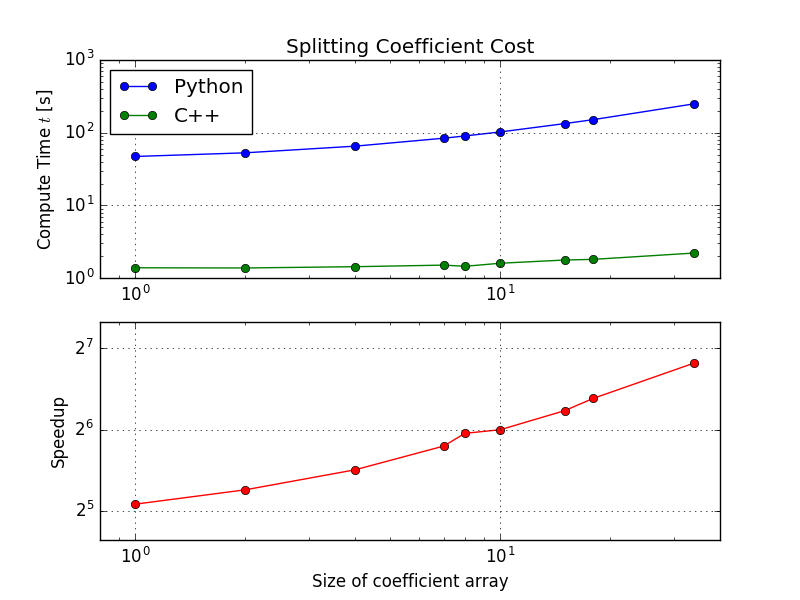
\includegraphics[width=.8\textwidth]{figures/coefs.png}
	\end{center}
	\caption{Comparison of computation times for different splitting coefficients $\{ w_T, w_U \}$ for Python code vs. C++ code. The absolute timings are shown in the top graph, the speedup on the bottom. It is remarkable that the initial speedup factor is about 30, but grows for larger coefficient sets. The speedup factor for the largest tested coefficient pair \emph{KL10} is over 110.
	All the timings in the table were measured by taking the average of 10 independent runs. The standard deviation of these measurements was below $1\%$ for the Python timings and below $0.1\%$ for the C++ timings. (Parameters: $1D$ torsional potential, $N=1$, $|\K|=16$ $\eps=0.01$, $T=10$, $\Dt=0.001$, Semiclassical propagator)}
	\label{fig:benchmarksplit}
\end{figure}


\subsubsection{Scaling with dimensionality D}
%
The question that was addressed in this benchmark is how the compute time of the code scales with increasing dimension $D$ of the wave packet.
Figure \ref{fig:dimension_analysis} shows a clear exponential scaling with the dimension $D$.
With a computation time of under 20 minutes for 100 time steps with the Semiclassical Propagator, dimension $D=5$ is still quite feasible.
%
\begin{figure}[ht]
	\centering
	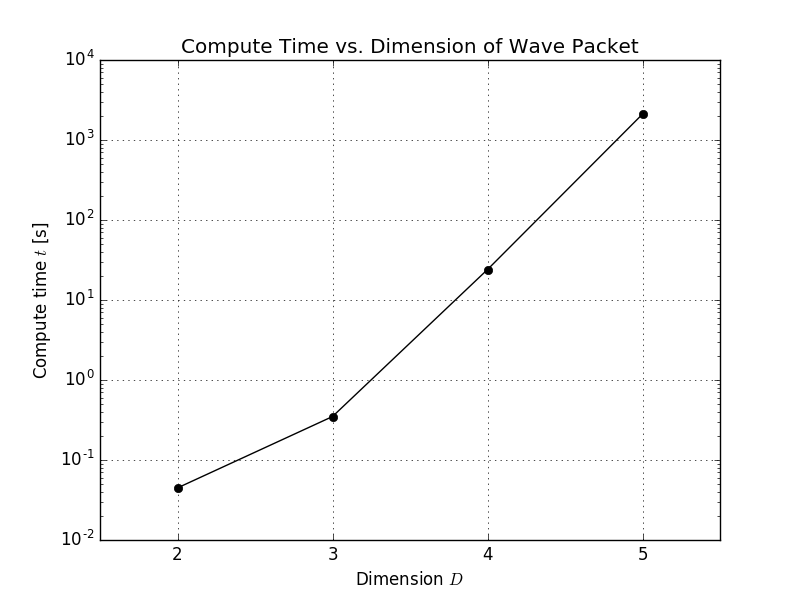
\includegraphics[width=.8\textwidth]{figures/dim.png}
	\caption{Scaling of the computation time with wave packet dimension $D$.
	(Parameters: $D$-dimensional torsional potential, $N=1$, $|\K|=4$ $\eps=0.01$, $T=1$, $\Dt=0.01$, Semiclassical propagator with \emph{LT} splitting for \proc{IntSplit})}
	\label{fig:dimension_analysis}
\end{figure}
